

\tikzset{every picture/.style={line width=0.75pt}} %set default line width to 0.75pt        

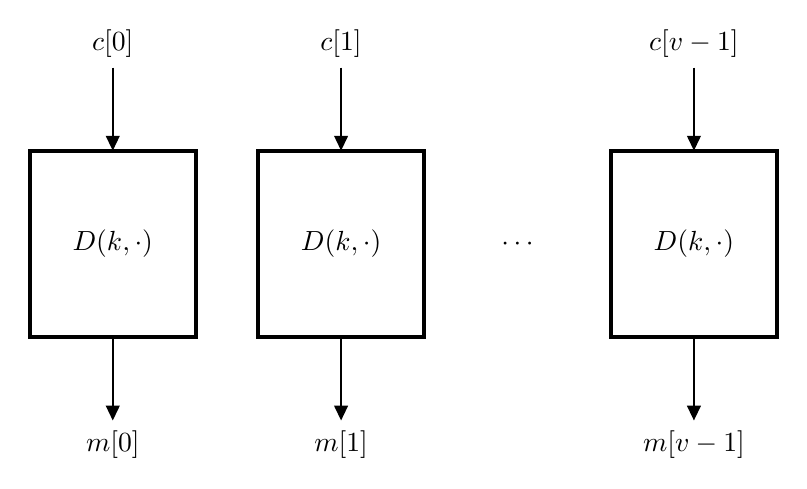
\begin{tikzpicture}[x=0.75pt,y=0.75pt,yscale=-1,xscale=1]
%uncomment if require: \path (0,248); %set diagram left start at 0, and has height of 248

%Shape: Rectangle [id:dp6289333122885685] 
\draw  [line width=1.5]  (0,80) -- (80,80) -- (80,170) -- (0,170) -- cycle ;
%Straight Lines [id:da22129734655304056] 
\draw    (40,40) -- (40,77) ;
\draw [shift={(40,80)}, rotate = 270] [fill={rgb, 255:red, 0; green, 0; blue, 0 }  ][line width=0.08]  [draw opacity=0] (7.14,-3.43) -- (0,0) -- (7.14,3.43) -- cycle    ;
%Straight Lines [id:da6968186105474381] 
\draw    (40,170) -- (40,207) ;
\draw [shift={(40,210)}, rotate = 270] [fill={rgb, 255:red, 0; green, 0; blue, 0 }  ][line width=0.08]  [draw opacity=0] (7.14,-3.43) -- (0,0) -- (7.14,3.43) -- cycle    ;
%Shape: Rectangle [id:dp6429978825026561] 
\draw  [line width=1.5]  (110,80) -- (190,80) -- (190,170) -- (110,170) -- cycle ;
%Straight Lines [id:da6636595423854752] 
\draw    (150,40) -- (150,77) ;
\draw [shift={(150,80)}, rotate = 270] [fill={rgb, 255:red, 0; green, 0; blue, 0 }  ][line width=0.08]  [draw opacity=0] (7.14,-3.43) -- (0,0) -- (7.14,3.43) -- cycle    ;
%Straight Lines [id:da35996083232833387] 
\draw    (150,170) -- (150,207) ;
\draw [shift={(150,210)}, rotate = 270] [fill={rgb, 255:red, 0; green, 0; blue, 0 }  ][line width=0.08]  [draw opacity=0] (7.14,-3.43) -- (0,0) -- (7.14,3.43) -- cycle    ;
%Shape: Rectangle [id:dp9712802234104969] 
\draw  [line width=1.5]  (280,80) -- (360,80) -- (360,170) -- (280,170) -- cycle ;
%Straight Lines [id:da003696637434867478] 
\draw    (320,40) -- (320,77) ;
\draw [shift={(320,80)}, rotate = 270] [fill={rgb, 255:red, 0; green, 0; blue, 0 }  ][line width=0.08]  [draw opacity=0] (7.14,-3.43) -- (0,0) -- (7.14,3.43) -- cycle    ;
%Straight Lines [id:da07604264241020542] 
\draw    (320,170) -- (320,207) ;
\draw [shift={(320,210)}, rotate = 270] [fill={rgb, 255:red, 0; green, 0; blue, 0 }  ][line width=0.08]  [draw opacity=0] (7.14,-3.43) -- (0,0) -- (7.14,3.43) -- cycle    ;

% Text Node
\draw (40,125) node    {$D( k,\cdot )$};
% Text Node
\draw (40,36.6) node [anchor=south] [inner sep=0.75pt]    {$c[ 0]$};
% Text Node
\draw (40,213.4) node [anchor=north] [inner sep=0.75pt]    {$m[ 0]$};
% Text Node
\draw (150,125) node    {$D( k,\cdot )$};
% Text Node
\draw (150,36.6) node [anchor=south] [inner sep=0.75pt]    {$c[ 1]$};
% Text Node
\draw (150,213.4) node [anchor=north] [inner sep=0.75pt]    {$m[ 1]$};
% Text Node
\draw (320,125) node    {$D( k,\cdot )$};
% Text Node
\draw (320,36.6) node [anchor=south] [inner sep=0.75pt]    {$c[ v-1]$};
% Text Node
\draw (320,213.4) node [anchor=north] [inner sep=0.75pt]    {$m[ v-1]$};
% Text Node
\draw (235,125) node    {$\cdots $};


\end{tikzpicture}